\documentclass[14pt]{extbook}
\usepackage{multicol, enumerate, enumitem, hyperref, color, soul, setspace, parskip, fancyhdr} %General Packages
\usepackage{amssymb, amsthm, amsmath, bbm, latexsym, units, mathtools} %Math Packages
\everymath{\displaystyle} %All math in Display Style
% Packages with additional options
\usepackage[headsep=0.5cm,headheight=12pt, left=1 in,right= 1 in,top= 1 in,bottom= 1 in]{geometry}
\usepackage[usenames,dvipsnames]{xcolor}
\usepackage{dashrule}  % Package to use the command below to create lines between items
\newcommand{\litem}[1]{\item#1\hspace*{-1cm}\rule{\textwidth}{0.4pt}}
\pagestyle{fancy}
\lhead{Progress Quiz 10}
\chead{}
\rhead{Version A}
\lfoot{6232-9639}
\cfoot{}
\rfoot{Fall 2020}
\begin{document}

\begin{enumerate}
\litem{
Solve the radical equation below. Then, choose the interval(s) that the solution(s) belongs to.\[ \sqrt{14 x^2 - 56} - \sqrt{33 x} = 0 \]\begin{enumerate}[label=\Alph*.]
\item \( x \in [3.4,5.4] \)
\item \( x_1 \in [-0.3, 2] \text{ and } x_2 \in [2.5,4.5] \)
\item \( x_1 \in [-1.7, -0.6] \text{ and } x_2 \in [2.5,4.5] \)
\item \( \text{All solutions lead to invalid or complex values in the equation.} \)
\item \( x \in [-1.7,-0.6] \)

\end{enumerate} }
\litem{
Solve the radical equation below. Then, choose the interval(s) that the solution(s) belongs to.\[ \sqrt{-6 x^2 - 6} - \sqrt{-13 x} = 0 \]\begin{enumerate}[label=\Alph*.]
\item \( \text{All solutions lead to invalid or complex values in the equation.} \)
\item \( x_1 \in [-0.51, 1.26] \text{ and } x_2 \in [-0.4,2.2] \)
\item \( x \in [1.42,1.95] \)
\item \( x_1 \in [-1.42, -0.2] \text{ and } x_2 \in [-2.7,0.6] \)
\item \( x \in [-0.51,1.26] \)

\end{enumerate} }
\litem{
Choose the graph of the equation below.\[ f(x) = - \sqrt{x - 14} + 3 \]\begin{enumerate}[label=\Alph*.]
\begin{multicols}{2}\item 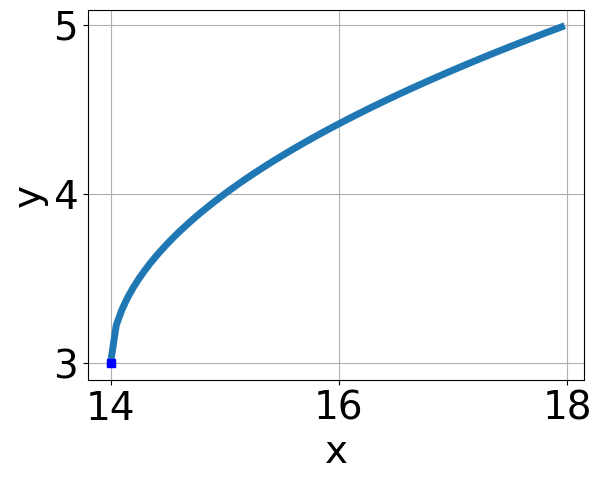
\includegraphics[width = 0.3\textwidth]{../Figures/radicalEquationToGraphCopyAA.png}\item 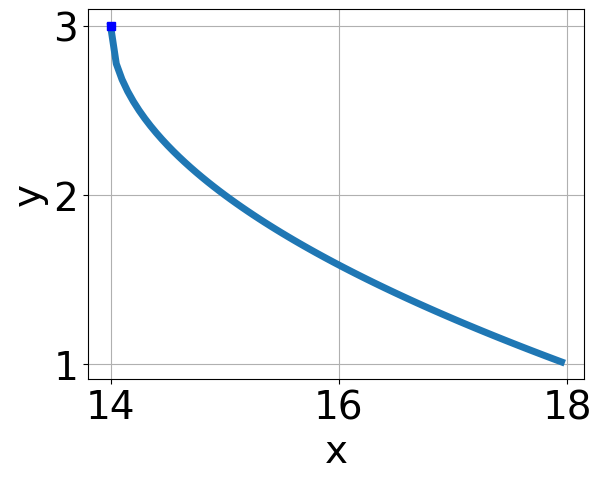
\includegraphics[width = 0.3\textwidth]{../Figures/radicalEquationToGraphCopyBA.png}\item 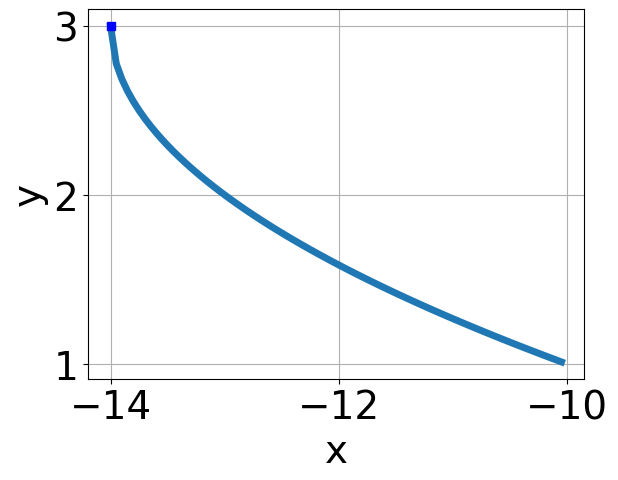
\includegraphics[width = 0.3\textwidth]{../Figures/radicalEquationToGraphCopyCA.png}\item 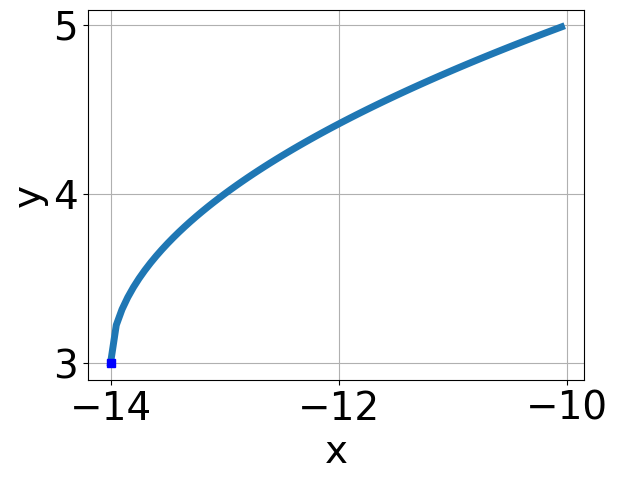
\includegraphics[width = 0.3\textwidth]{../Figures/radicalEquationToGraphCopyDA.png}\end{multicols}\item None of the above.
\end{enumerate} }
\litem{
What is the domain of the function below?\[ f(x) = \sqrt[7]{3 x + 5} \]\begin{enumerate}[label=\Alph*.]
\item \( \text{The domain is } (-\infty, a], \text{   where } a \in [-0.63, -0.35] \)
\item \( \text{The domain is } [a, \infty), \text{   where } a \in [-2.13, -1.01] \)
\item \( \text{The domain is } [a, \infty), \text{   where } a \in [-0.72, 1.58] \)
\item \( \text{The domain is } (-\infty, a], \text{   where } a \in [-2.85, -1.22] \)
\item \( (-\infty, \infty) \)

\end{enumerate} }
\litem{
Choose the graph of the equation below.\[ f(x) = - \sqrt{x - 6} - 5 \]\begin{enumerate}[label=\Alph*.]
\begin{multicols}{2}\item 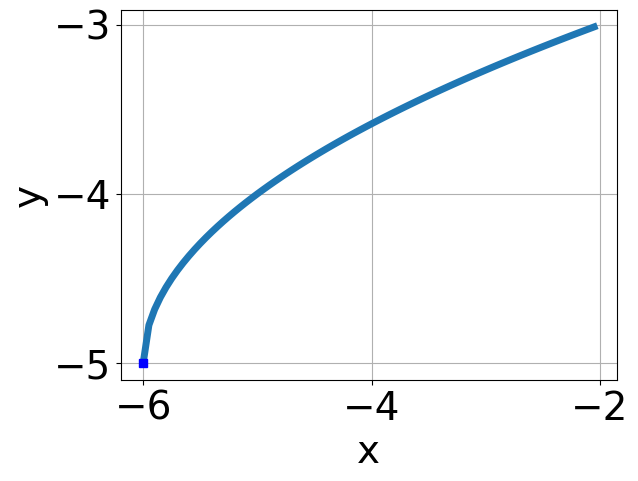
\includegraphics[width = 0.3\textwidth]{../Figures/radicalEquationToGraphAA.png}\item 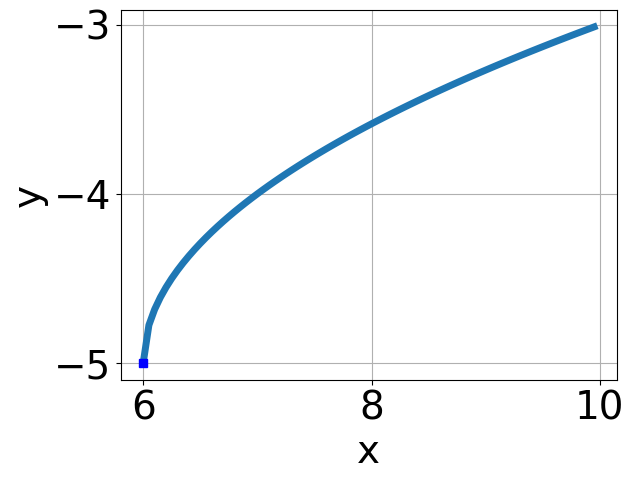
\includegraphics[width = 0.3\textwidth]{../Figures/radicalEquationToGraphBA.png}\item 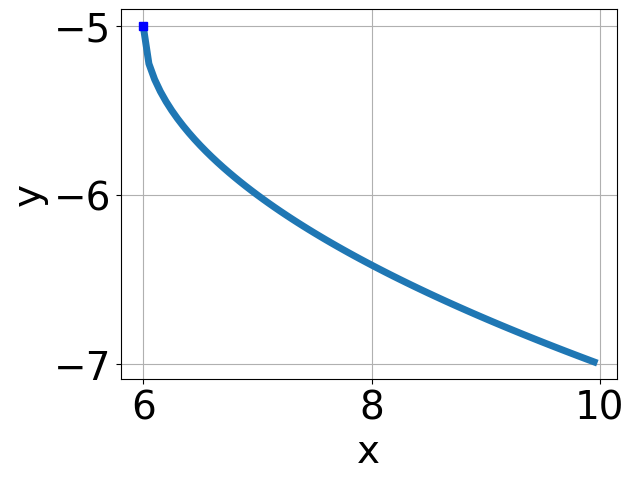
\includegraphics[width = 0.3\textwidth]{../Figures/radicalEquationToGraphCA.png}\item 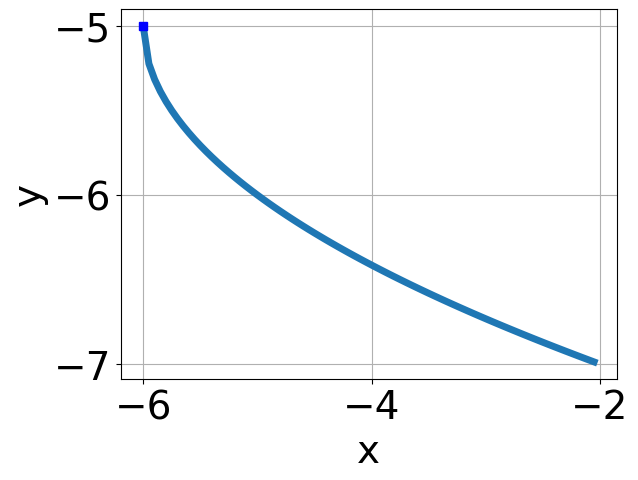
\includegraphics[width = 0.3\textwidth]{../Figures/radicalEquationToGraphDA.png}\end{multicols}\item None of the above.
\end{enumerate} }
\litem{
Choose the equation of the function graphed below.
\begin{center}
    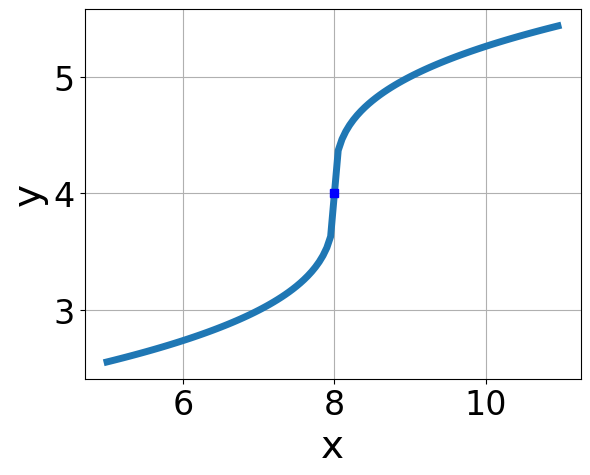
\includegraphics[width=0.5\textwidth]{../Figures/radicalGraphToEquationA.png}
\end{center}
\begin{enumerate}[label=\Alph*.]
\item \( f(x) = - \sqrt[3]{x + 8} + 4 \)
\item \( f(x) = - \sqrt[3]{x - 8} + 4 \)
\item \( f(x) = \sqrt[3]{x - 8} + 4 \)
\item \( f(x) = \sqrt[3]{x + 8} + 4 \)
\item \( \text{None of the above} \)

\end{enumerate} }
\litem{
Solve the radical equation below. Then, choose the interval(s) that the solution(s) belongs to.\[ \sqrt{-2 x - 7} - \sqrt{8 x - 6} = 0 \]\begin{enumerate}[label=\Alph*.]
\item \( x_1 \in [-3.72, -2.78] \text{ and } x_2 \in [-0.53,0.47] \)
\item \( x \in [-1.89,-0.2] \)
\item \( x \in [-0.86,0.62] \)
\item \( \text{All solutions lead to invalid or complex values in the equation.} \)
\item \( x_1 \in [-3.72, -2.78] \text{ and } x_2 \in [0.58,1.06] \)

\end{enumerate} }
\litem{
Solve the radical equation below. Then, choose the interval(s) that the solution(s) belongs to.\[ \sqrt{-5 x - 5} - \sqrt{-4 x + 7} = 0 \]\begin{enumerate}[label=\Alph*.]
\item \( x_1 \in [-13.2, -10.1] \text{ and } x_2 \in [-3,1] \)
\item \( x \in [-13.2,-10.1] \)
\item \( \text{All solutions lead to invalid or complex values in the equation.} \)
\item \( x_1 \in [-1.4, 1.2] \text{ and } x_2 \in [-0.25,4.75] \)
\item \( x \in [1.9,2.7] \)

\end{enumerate} }
\litem{
What is the domain of the function below?\[ f(x) = \sqrt[4]{4 x - 9} \]\begin{enumerate}[label=\Alph*.]
\item \( (-\infty, \infty) \)
\item \( [a, \infty), \text{ where } a \in [1.8, 2.7] \)
\item \( [a, \infty), \text{where } a \in [0, 2.2] \)
\item \( (-\infty, a], \text{where } a \in [-1.3, 1.2] \)
\item \( (-\infty, a], \text{where } a \in [0.9, 3.1] \)

\end{enumerate} }
\litem{
Choose the equation of the function graphed below.
\begin{center}
    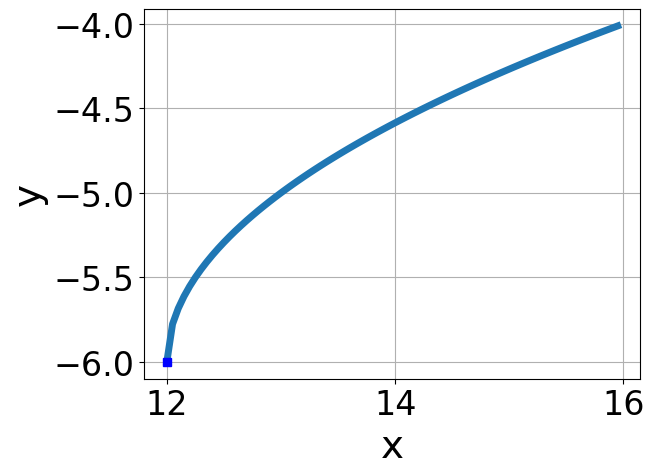
\includegraphics[width=0.5\textwidth]{../Figures/radicalGraphToEquationCopyA.png}
\end{center}
\begin{enumerate}[label=\Alph*.]
\item \( f(x) = \sqrt[3]{x - 12} - 6 \)
\item \( f(x) = - \sqrt[3]{x - 12} - 6 \)
\item \( f(x) = - \sqrt[3]{x + 12} - 6 \)
\item \( f(x) = \sqrt[3]{x + 12} - 6 \)
\item \( \text{None of the above} \)

\end{enumerate} }
\end{enumerate}

\end{document}